%Version 3.1 December 2024
% See section 11 of the User Manual for version history
%
%%%%%%%%%%%%%%%%%%%%%%%%%%%%%%%%%%%%%%%%%%%%%%%%%%%%%%%%%%%%%%%%%%%%%%
%%                                                                 %%
%% Please do not use \input{...} to include other tex files.       %%
%% Submit your LaTeX manuscript as one .tex document.              %%
%%                                                                 %%
%% All additional figures and files should be attached             %%
%% separately and not embedded in the \TeX\ document itself.       %%
%%                                                                 %%
%%%%%%%%%%%%%%%%%%%%%%%%%%%%%%%%%%%%%%%%%%%%%%%%%%%%%%%%%%%%%%%%%%%%%

%%\documentclass[referee,sn-basic]{sn-jnl}% referee option is meant for double line spacing

%%=======================================================%%
%% to print line numbers in the margin use lineno option %%
%%=======================================================%%

%%\documentclass[lineno,pdflatex,sn-basic]{sn-jnl}% Basic Springer Nature Reference Style/Chemistry Reference Style

%%=========================================================================================%%
%% the documentclass is set to pdflatex as default. You can delete it if not appropriate.  %%
%%=========================================================================================%%

%%\documentclass[sn-basic]{sn-jnl}% Basic Springer Nature Reference Style/Chemistry Reference Style

%%Note: the following reference styles support Namedate and Numbered referencing. By default the style follows the most common style. To switch between the options you can add or remove “Numbered” in the optional parenthesis. 
%%The option is available for: sn-basic.bst, sn-chicago.bst%  
 
%%\documentclass[pdflatex,sn-nature]{sn-jnl}% Style for submissions to Nature Portfolio journals
\documentclass[pdflatex,sn-basic]{sn-jnl}% Basic Springer Nature Reference Style/Chemistry Reference Style
%\documentclass[pdflatex,sn-mathphys-num]{sn-jnl}% Math and Physical Sciences Numbered Reference Style
%%\documentclass[pdflatex,sn-mathphys-ay]{sn-jnl}% Math and Physical Sciences Author Year Reference Style
%%\documentclass[pdflatex,sn-aps]{sn-jnl}% American Physical Society (APS) Reference Style
%\documentclass[pdflatex,sn-vancouver-num]{sn-jnl}% Vancouver Numbered Reference Style
%%\documentclass[pdflatex,sn-vancouver-ay]{sn-jnl}% Vancouver Author Year Reference Style
%\documentclass[pdflatex,sn-apa]{sn-jnl}% APA Reference Style
%%\documentclass[pdflatex,sn-chicago]{sn-jnl}% Chicago-based Humanities Reference Style

%%%% Standard Packages
%%<additional latex packages if required can be included here>

\usepackage{graphicx}%
\usepackage{multirow}%
\usepackage{amsmath,amssymb,amsfonts}%
\usepackage{amsthm}%
\usepackage{mathrsfs}%
\usepackage[title]{appendix}%
\usepackage{xcolor}%
\usepackage{textcomp}%
\usepackage{manyfoot}%
\usepackage{booktabs}%
\usepackage{algorithm}%
\usepackage{algorithmicx}%
\usepackage{algpseudocode}%
\usepackage{listings}%
\usepackage{url}%
%%%%

%%%%%=============================================================================%%%%
%%%%  Remarks: This template is provided to aid authors with the preparation
%%%%  of original research articles intended for submission to journals published 
%%%%  by Springer Nature. The guidance has been prepared in partnership with 
%%%%  production teams to conform to Springer Nature technical requirements. 
%%%%  Editorial and presentation requirements differ among journal portfolios and 
%%%%  research disciplines. You may find sections in this template are irrelevant 
%%%%  to your work and are empowered to omit any such section if allowed by the 
%%%%  journal you intend to submit to. The submission guidelines and policies 
%%%%  of the journal take precedence. A detailed User Manual is available in the 
%%%%  template package for technical guidance.
%%%%%=============================================================================%%%%

%% as per the requirement new theorem styles can be included as shown below
\theoremstyle{thmstyleone}%
\newtheorem{theorem}{Theorem}%  meant for continuous numbers
%%\newtheorem{theorem}{Theorem}[section]% meant for sectionwise numbers
%% optional argument [theorem] produces theorem numbering sequence instead of independent numbers for Proposition
\newtheorem{proposition}[theorem]{Proposition}% 
%%\newtheorem{proposition}{Proposition}% to get separate numbers for theorem and proposition etc.

\theoremstyle{thmstyletwo}%
\newtheorem{example}{Example}%
\newtheorem{remark}{Remark}%

\theoremstyle{thmstylethree}%
\newtheorem{definition}{Definition}%

\raggedbottom
%%\unnumbered% uncomment this for unnumbered level heads

\begin{document}

\title[Article Title]{The Fabricated Front: GenAI and the Social Organization of Workplace Legibility}

%%=============================================================%%
%% GivenName	-> \fnm{Joergen W.}
%% Particle	-> \spfx{van der} -> surname prefix
%% FamilyName	-> \sur{Ploeg}
%% Suffix	-> \sfx{IV}
%% \author*[1,2]{\fnm{Joergen W.} \spfx{van der} \sur{Ploeg} 
%%  \sfx{IV}}\email{iauthor@gmail.com}
%%=============================================================%%

\author*[1,2]{\fnm{Tom} \sur{Van Nuenen}}\email{tomvannuenen@berkeley.edu}

\author[2,3]{\fnm{Pratik} \sur{S. Sachdeva}}\email{pratik.sachdeva@berkeley.edu}

\author[1,2]{\fnm{Sahiba} \sur{Chopra}}\email{sahiba.chopra@berkeley.edu}

\affil*[1]{\orgdiv{D-Lab}, \orgname{University of California, Berkeley}, \orgaddress{\street{356 Social Science Building}, \city{Berkeley}, \postcode{94720}, \state{CA}, \country{USA}}}

\affil[2]{\orgdiv{D-Lab}, \orgname{University of California, Berkeley}, \orgaddress{\street{356 Social Science Building}, \city{Berkeley}, \postcode{94720}, \state{CA}, \country{USA}}}

\affil[3]{\orgdiv{Haas School of Business}, \orgname{University of California, Berkeley}, \orgaddress{\street{2220 Piedmont Avenue}, \city{Berkeley}, \postcode{94720}, \state{CA}, \country{USA}}}

%%==================================%%
%% Sample for unstructured abstract %%
%%==================================%%

\abstract{Generative AI (GenAI) has become a fixture of workplace life. Current research asks chiefly what this implies for jobs and outputs, measured in productivity, displacement, or bias. What remains underexamined are the interactional reconfigurations that GenAI produces at work. Chopra’s (2026) theory of effort opacity has begun to fill this gap by noting the systematic decoupling of observable output from human engagement. When GenAI makes interactional cues less diagnostic, it weakens the reciprocal exchange that sustains collaborative trust. Extending this account of effort opacity, we examine the interactional mechanics that produce opacity in everyday workplace encounters. 

Drawing on Erving Goffman's dramaturgical framework and 1,250 interview transcripts from Anthropic's AI Interviewer dataset, we identify five opacity mechanisms through which workplace fronts are reorganized: voice, vulnerability, provenance, attention, and investment opacity. We show that professionals defend identity opacity (voice, provenance) while freely producing labor opacity (vulnerability, attention, investment), and we trace this asymmetry to its forensic logic: identity cues leave auditable signatures while labor cues do not. The governance task, accordingly, is one of involvement management: specifying which forms of human involvement (attention, effort, judgment) must remain inspectable, and to whom. Workplace AI policies built on universal disclosure will systematically misrecognize a social field in which inspectability is already audience-relative.}

%%================================%%
%% Sample for structured abstract %%
%%================================%%

% \abstract{\textbf{Purpose:} The abstract serves both as a general introduction to the topic and as a brief, non-technical summary of the main results and their implications. The abstract must not include subheadings (unless expressly permitted in the journal's Instructions to Authors), equations or citations. As a guide the abstract should not exceed 200 words. Most journals do not set a hard limit however authors are advised to check the author instructions for the journal they are submitting to.
% 
% \textbf{Methods:} The abstract serves both as a general introduction to the topic and as a brief, non-technical summary of the main results and their implications. The abstract must not include subheadings (unless expressly permitted in the journal's Instructions to Authors), equations or citations. As a guide the abstract should not exceed 200 words. Most journals do not set a hard limit however authors are advised to check the author instructions for the journal they are submitting to.
% 
% \textbf{Results:} The abstract serves both as a general introduction to the topic and as a brief, non-technical summary of the main results and their implications. The abstract must not include subheadings (unless expressly permitted in the journal's Instructions to Authors), equations or citations. As a guide the abstract should not exceed 200 words. Most journals do not set a hard limit however authors are advised to check the author instructions for the journal they are submitting to.
% 
% \textbf{Conclusion:} The abstract serves both as a general introduction to the topic and as a brief, non-technical summary of the main results and their implications. The abstract must not include subheadings (unless expressly permitted in the journal's Instructions to Authors), equations or citations. As a guide the abstract should not exceed 200 words. Most journals do not set a hard limit however authors are advised to check the author instructions for the journal they are submitting to.}

\keywords{Generative AI, Workplace communication, Effort opacity, Interactional opacity, Workplace trust, AI-mediated communication, Professional identity}

%%\pacs[JEL Classification]{D8, H51}

%%\pacs[MSC Classification]{35A01, 65L10, 65L12, 65L20, 65L70}

\maketitle

% ============================================================================
% 1. INTRODUCTION
% ============================================================================
\section{Introduction}

Workplace trust depends on the everyday interpretation of communicative performances. When a colleague sends an email or delivers a report, we make inferences about the person behind the performance. Word choice signals attentiveness, for instance, and distinctive phrasing indexes personality. These diagnostic cues form the tacit infrastructure of workplace coordination, helping us allocate trust and calibrate expectations. In other words, professional communication functions as a ``front,’’ a patterned performance through which workers make competence and commitment available for interpretation \citep{goffman1959presentation}. Generative AI (GenAI) disrupts this infrastructure by introducing a new form of mediated communication in which a system can modify, augment, or generate interpersonal messages on behalf of a communicator \citep{hancock2020aimediated}. When outputs can be produced without the engagement they appear to represent, the interpretive framework through which we read professional contributions becomes unreliable.

This paper examines how professionals navigate the use of an AI-mediated front. We take as our starting point Chopra's concept of ``effort opacity,'' the systematic decoupling of observable output from human engagement \citep{chopra2026engagement}. When GenAI makes interactional cues less diagnostic, it weakens the reciprocal exchange that sustains collaborative trust. A remaining question is how professionals decide which forms of legibility to preserve and how those choices reorganize accountability in everyday work.

Prior work has shown that AI use can carry reputational costs and create a transparency dilemma, in which disclosure may reduce rather than restore trust \citep{schilke2025transparency, reif2025social}. We extend these accounts through a typology of opacity mechanisms, 
each describing an inference audiences ordinarily draw from a worker's front that AI usage now disrupts.
Drawing on Erving Goffman's dramaturgical framework, we argue that GenAI fundamentally alters the shared assumptions about who is speaking in what capacity, what commitments utterances carry, and what counts as evidence of engagement \citep{goffman1959presentation}. 
We analyze 1,250 interview transcripts from Anthropic's AI Interviewer dataset, capturing professionals across the general workforce, the creative industry, and the sciences. We show how these workers resist opacity around identity mechanisms (who one appears to be), yet freely produce it around labor mechanisms (what one actually did). We argue that AI policies that ignore the audience structure of inspectability will produce compliant disclosures, while the concealment they aim to address will continue.


% ============================================================================
% 2. FROM EFFORT OPACITY TO INTERACTIONAL OPACITY
% ============================================================================
\section{From Effort Opacity to Interactional Opacity}

Erving Goffman's dramaturgical sociology treats social life as performances in which actors control the impressions they convey \citep{goffman1959presentation}. Central is the ``definition of the situation'': an understanding, shared by participants, about what kind of interaction is taking place, who is participating in what capacity, and what standards of conduct therefore apply \citep{goffman1974frame}. In workplace settings, this includes assumptions about whether an email, report, or comment reflects a person's own judgment, how much thought or attention it represents, and what kind of accountability attaches to it.

To specify how GenAI unsettles this definition of the situation, we draw on three related Goffmanian concepts. First, \textit{footing} describes speakers' alignment toward utterances \citep{goffman1981forms}. Goffman distinguishes the \textit{animator} (who produces an utterance), the \textit{author} (who composes it), and the \textit{principal} (whose position it establishes). These roles, Goffman noted, are routinely separable in institutional contexts: a press secretary, for instance, animates words composed by speechwriters on behalf of the office they represent. Such signals, like a podium with the presidential seal, mark the decoupling. Generative AI inserts it into ordinary contexts where no such signals exist and author and animator are assumed identical. 

Second, \textit{front stage} and \textit{back stage} capture how performers manage information across regions visible and invisible to the audience. Goffman's example of a back stage is a collective space where teammates coordinate and rehearse for the front stage performance. AI enters this region as a substitute for the teammates who would have otherwise been there, and as a shared resource among peers. In both cases, GenAI reshapes what front stage performances seem to reveal about the labor behind them. Third, \textit{stigma} examines how individuals manage potentially discrediting attributes \citep{goffman1963stigma}. Emerging evidence suggests AI use is becoming such an attribute in some professional settings, resulting in strategic concealment \citep{schilke2025transparency}.

A dominant strand of research measures AI's effect on workplace output and reports productivity gains across writing tasks \citep{noy2023experimental}, knowledge-worker projects \citep{dellacqua2023navigating}, and customer service work \citep{brynjolfsson2025generative}. A consistent finding across these studies is that less-experienced workers gain the most in using AI. Yet these are also the workers whose unaided competence is most under scrutiny, and who therefore have the most reason to conceal AI use. A growing complementary literature documents this side of the picture. Workers anticipate and receive negative judgments around competence and motivation \citep{reif2025social}, and disclosure can paradoxically reduce trust rather than restore it \citep{schilke2025transparency}. They respond by hiding AI use from those whose judgments they fear (managers, evaluators) while remaining open with peers \citep{xia2026clever}. The same passing dynamic extends beyond conventional workplaces. In China's short-video creator economy, content creators perform substantial editing of AI outputs to pass them as human-authored, in what the authors call \textit{invisible authenticity labor} \citep{su2026passing}.

Work on authorship and credit attribution adds further detail. Knowledge workers systematically discount AI contributions relative to human ones and place strong normative weight on disclosure \citep{he2025credit}, while AI-assisted writing increases productivity yet reduces users' sense of accountability for the resulting text \citep{li2024writing}. \citet{chopra2026engagement} synthesizes these strands. As AI makes outputs easier to produce, observable performance becomes less diagnostic of engagement, and contributions exhibiting ``AI signatures'' face higher rejection rates and less developmental feedback. In parallel, HCI research shows that AI-generated meeting summaries restructure attention and organizational memory \citep{asthana2025meeting}, prompting calls to study collective coordination rather than individual productivity \citep{woolley2025collaboration}.

This body of work establishes that AI use is absorbed into the labor of seeming authentic. The closest dramaturgical reading is \citet{klowait2025presentation}, who reframe AI as supplementary rather than substitutive automation: LLMs absorb the invisible, routine tasks of cognitive work (such as editing or summarizing) while humans enact the visible, relational facets that sustain professional prestige. We extend this empirically, tracing how workers navigate the new AI-human division of labor.

Goffman's framework lets us name three features of ordinary workplace performance, and our close readings in \S 4 show each being undercut by GenAI. The social occasions Goffman describes, such as the moments when suspicion leads to repair or novice uncertainty becomes an opportunity for instruction, dissolve before they can happen. Footing splits across time, with workers using GenAI to animate, in the present, what an archived version of themselves would have written. And what Goffman treats as a continuous stream of small choices collapses into a single founding decision. We will argue these breaks reframe the analytic problem from impression management to what we will call \textit{involvement management}: the practical question of which forms of human involvement must remain inspectable for the performance to count as the worker's own.

A key implication running throughout the analysis is that the opacity of labor should not be mistaken for its disappearance. In many cases, the labor AI removes from the visible artifact reappears as invisible upkeep---prompting, checking, hedging, and repairing the cue surface---redirecting effort from producing the output to maintaining the conditions under which it still reads as the worker's own.


% ============================================================================
% 3. FIVE OPACITY MECHANISMS
% ============================================================================
\section{Five Opacity Mechanisms}

Building on Chopra's effort opacity, i.e. the general decoupling of output from human engagement, we describe five mechanisms that specify where the decoupling occurs.

\textit{Voice opacity} concerns the filtering of stance cues and footing: AI-mediated text may be eloquent but no longer indexes the person who sent it, removing both the personality cues through which colleagues recognize one another \citep{hyland2012disciplinary} and the situational cues (mood, urgency, hesitation) that signal how they are approaching the encounter. \textit{Vulnerability opacity} emerges when AI handles uncertainty for workers, filtering out the hedges and pauses that ordinarily invite mentorship \citep{edmondson1999psychological}. \textit{Provenance opacity} describes gaps in accountability when workers cannot reconstruct the reasoning behind AI-assisted artifacts; the report may appear defensible until others demand explanation or repair. \textit{Attention opacity} decouples interactional participation from cognitive engagement, with AI summarizers and meeting assistants letting workers perform attendance without attention while reshaping the official memory of events \citep{suchman1987plans}. \textit{Investment opacity} describes the process of high- and low-investment outputs becoming indistinguishable, shifting the basis for credit from demonstrated work to inferences about character and motive.

The five mechanisms are not parallel choices. Voice and provenance index who one appears to be: the personality and authorial stance audiences read from a worker's cue surface. Vulnerability, attention, and investment index what one actually did: the engagement, attentiveness, and effort the worker brought to the artifact. The typology specifies what existing accounts treat as undifferentiated. These mechanisms differ in terms of which audiences can detect them, in what kinds of evidence they leave behind, and in how workers strategically prioritize them. 

% ============================================================================
% 4. EVIDENCE FROM THE INTERVIEW CORPUS
% ============================================================================
\section{Evidence from the Interview Corpus}

To examine how workers themselves decide which forms of AI mediation are acceptable or worth concealing, we analyze 1,250 transcripts from Anthropic's AI Interviewer dataset \citep{anthropic2025interviewer}, comprising general workforce participants ($n = 1{,}000$), creative professionals ($n = 125$), and scientists ($n = 125$). Participants were recruited through crowdworker platforms. The general workforce sample is led by education and instruction (17\%), computing and mathematics (16\%), and arts, design, and media (14\%); the creative sample by writers and authors (48\%) and visual artists (21\%); and the scientist sample spans fifty-plus disciplines, with physics, chemistry, and chemical engineering best represented. Each interview is a 10--15 minute semi-structured conversation conducted by Claude, following a question plan that Anthropic researchers reviewed and finalized before deployment, that probes participants' experiences integrating generative AI into their work. Participants provided informed consent for public release; transcripts are distributed under CC-BY.

We used LLM-assisted coding (GPT-5.4 with ``medium'' reasoning effort) to classify each transcript by our theoretical framework. For each opacity mechanism, we assessed \textit{salience} (none, potential, clear) and \textit{behavioral orientation} (production, avoidance, mixed). To capture practical reasoning, we hand-coded a stratified sample of 207 cases for justification type, distinguishing accountability-oriented justifications (invoking responsibility, liability, and professional obligation) from efficiency-oriented justifications (invoking time-saving and productivity). These categories are not mutually exclusive.

Salience marks the mechanism's presence in the transcript: \textit{absent} when the participant does not describe anything related to it; \textit{potential} when the participant describes an activity that could surface as opacity given the right interactional conditions but does not explicitly name it as such; and \textit{clear} when the participant explicitly names the opacity concern.
 
Behavioral orientation captures the participant's stance toward the mechanism. \textit{Avoidance} describes practices that resist producing opacity, such as a worker editing AI output to sound like themselves before sending. \textit{Production} describes practices that create or allow opacity, such as a worker delegating the cue surface to AI without correction. Mixed cases include both within the same account. A worker who consistently rewrites AI-drafted emails to preserve their style codes as voice opacity, clear, avoidance. One who sends
AI-generated text without editing codes as clear production. One who uses AI for emails without addressing whether the resulting text reflects their voice codes as potential.

Group differences in mechanism prevalence and behavioral orientation were tested using Pearson's chi-squared tests of independence. Pairwise post-hoc comparisons used chi-squared tests with Yates' continuity correction and Bonferroni adjustment across three comparisons.

\subsection{Mechanism Prevalence and Variation Across Groups}

LLM-assisted coding reveals that opacity concerns pervade professionals' accounts but vary substantially in salience (Figure~\ref{fig:prevalence}). Voice opacity is most prevalent (61.8\% of transcripts), followed by provenance (45.1\%), investment (38.1\%), vulnerability (30.4\%), and attention (9.4\%). Attention's rarity reflects both the recency of AI meeting tools and the narrower range of tasks where engagement can be meaningfully delegated. Where it does appear, accounts frame delegation as efficiency rather than evasion, contrasting with the moral vocabulary that surrounds other mechanisms.

\begin{figure}[htbp]
\centering
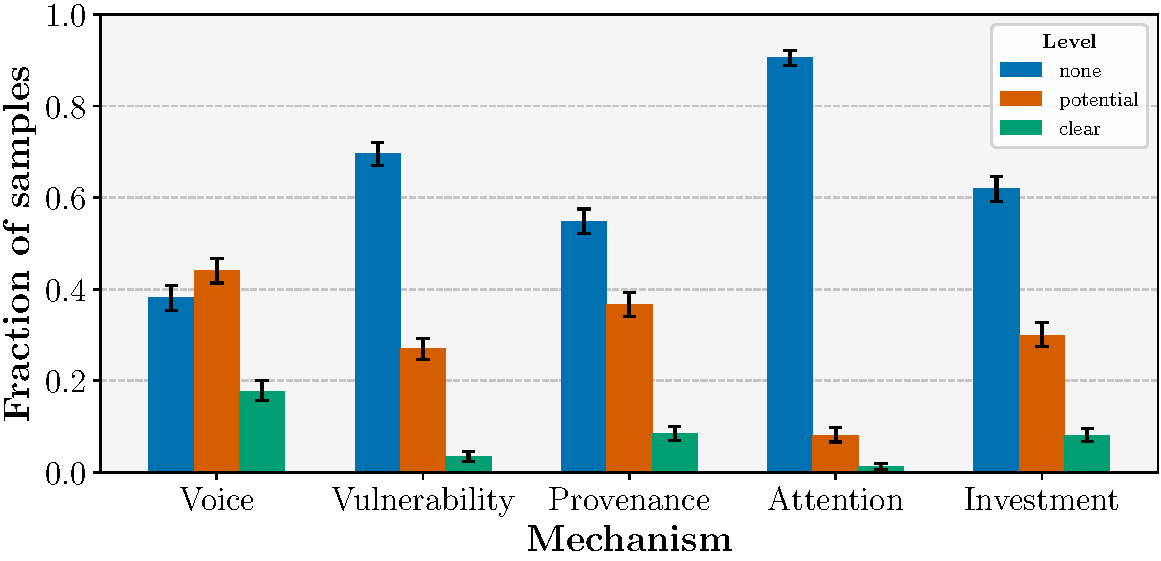
\includegraphics[width=0.9\textwidth]{figures/all_interview_opacity.pdf}
\caption{Prevalence of opacity mechanisms across all interviews ($N = 1,250$). Bars show fraction of transcripts at each level (none, potential, clear).}
\label{fig:prevalence}
\end{figure}

Beyond corpus-wide prevalence, the specific mechanisms that professionals discuss vary systematically by domain (Figure~\ref{fig:groups}). Voice opacity was most prevalent among general workforce participants (66.4\%) and creative professionals (56.8\%), and notably lower among scientists (30.4\%; $\chi^2 = 62.52$, $p < .001$). Post-hoc pairwise comparisons confirm that scientists differ significantly from both other groups (vs. workforce, $p < .001$; vs. creatives, $p < .001$), while workforce and creatives do not differ significantly from each other ($p = 0.13$). The split runs primarily between scientific and non-scientific work.

Provenance opacity showed the inverse pattern. It was highest among scientists (75.2\%), moderate in the workforce (44.2\%), and lowest among creatives (22.4\%; $\chi^2 = 72.08$, $p < .001$, with all three pairwise differences significant after Bonferroni correction, $p < .001$). One scientist captured the logic in their interview: ``I will ask for references and then check them\ldots about half the time the AI will give quotes that don't exist. The possibility of nonsense means I can't send an application in, as it will be reviewed by people who know the subject'' [science\_0121].

Investment opacity was most prevalent among creative professionals (58.4\%), compared to 38.4\% in the workforce and 15.2\% among scientists ($\chi^2 = 49.68$, $p < .001$, with all three pairwise differences significant after Bonferroni correction, $p < .001$). Governance frameworks around credit and compensation in creative AI work remain contested \citep{chi2025creative}.

These group differences likely reflect what each field treats as the cue surface of professional credibility. Scientific writing rewards evidentiary restraint over expressive individuality; creative fields valorize visible craft and effort; workforce communication depends on distinctive style as a signal of engagement. Workers tend to defend the mechanism whose loss would most damage their domain's specific credibility infrastructure.

\begin{figure}[htbp]
\centering
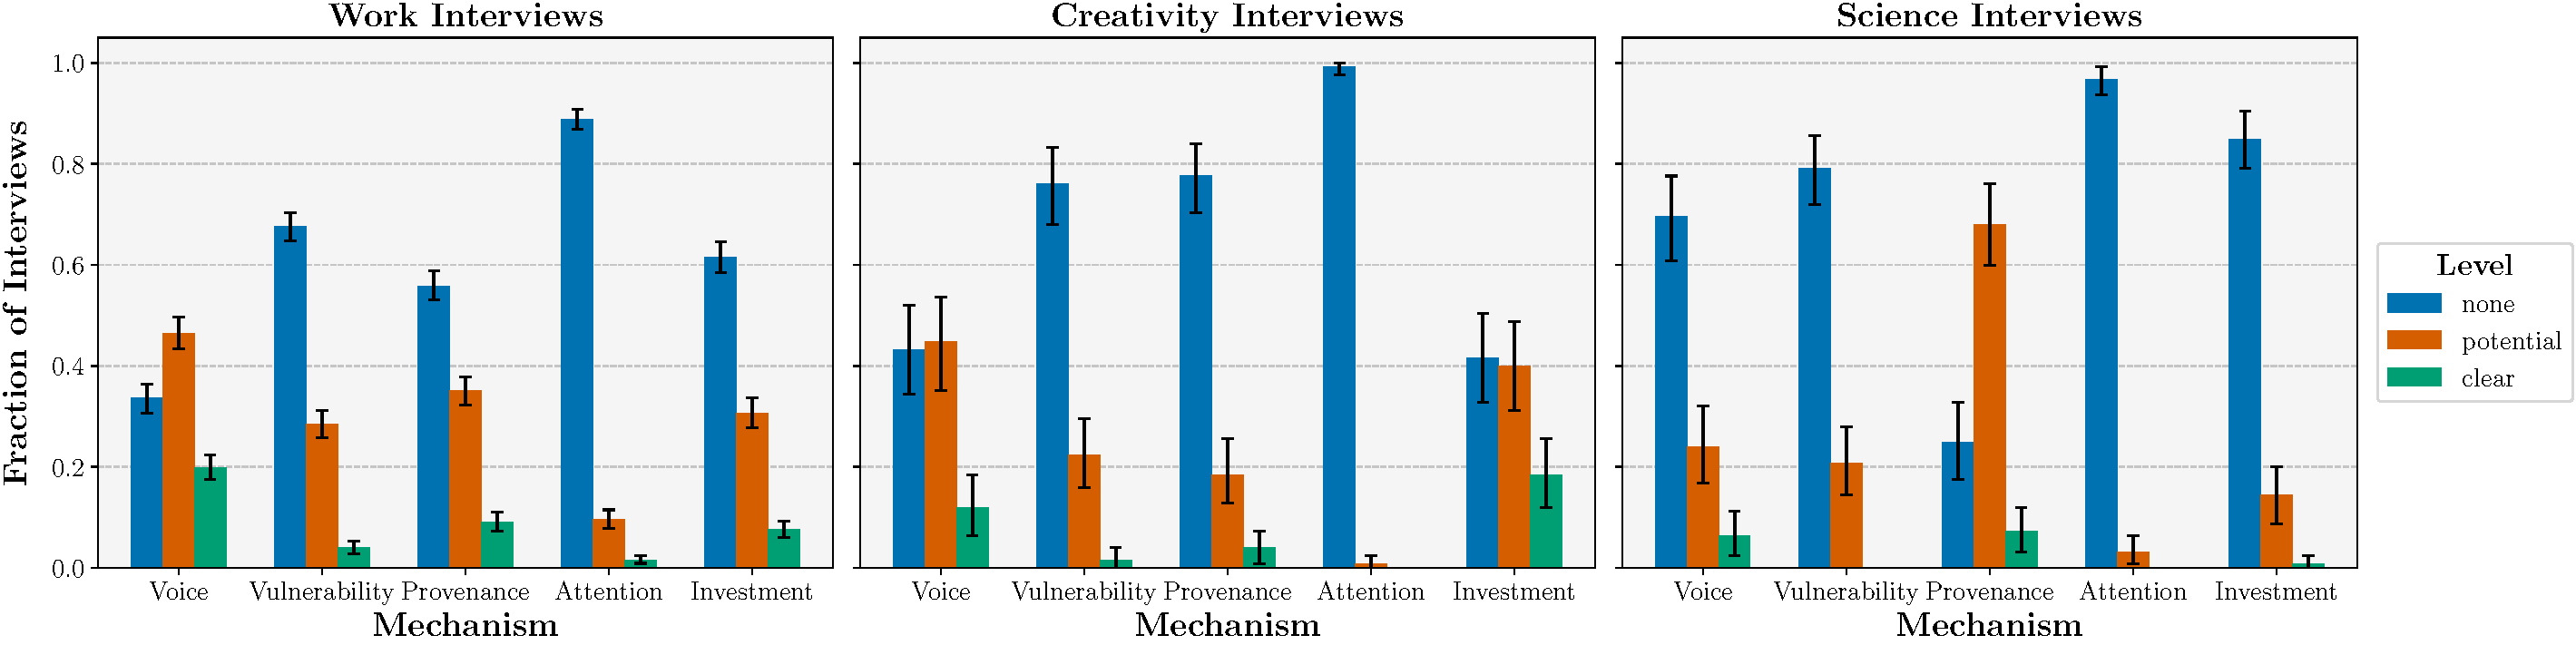
\includegraphics[width=0.9\textwidth]{figures/interview_mechanism_by_type.pdf}
\caption{Opacity mechanisms by professional group.}
\label{fig:groups}
\end{figure}

\subsection{Identity/Labor Asymmetry}

Beyond prevalence, the most striking finding is in workers' behavioral orientation, which varies dramatically by mechanism type. Figure~\ref{fig:form} displays the distribution of production, avoidance, and mixed orientations across mechanisms.

Provenance opacity showed the highest avoidance:production ratio at 1.39:1 (avoidance cases per production case), the only mechanism where avoidance exceeded production overall. This aggregate is driven by scientists (9:1) and workforce (1.2:1); for creatives the ratio inverts (0.5:1, $n = 28$), consistent with provenance's lower role in creative credibility infrastructure. When professionals defend provenance, they describe practices that preserve their capacity to stand behind the work, such as verification, citation-checking, or refusal to sign material they have not finalized.

The labor-relevant mechanisms, however, present a different picture. Vulnerability opacity was near-universally produced: 93.2\% of cases involved creating or allowing opacity, with only 1.8\% avoidance (ratio 0.02:1). Participants described hiding knowledge gaps and presenting façades of competence with little apparent concern. Investment opacity followed the same pattern, with 82.4\% production against 5.5\% avoidance (ratio 0.07:1). Cases such as the software developer who ``had AI do all the work'' while appearing to ``lead'' the project were common and largely unreflective. Attention opacity, though rarer overall, was also predominantly produced (65.0\% production, 14.5\% avoidance, ratio 0.22:1).

The pattern aligns with the identity/labor distinction introduced in \S 3. Identity mechanisms (voice, provenance) showed 464 cases of production against 344 of avoidance (ratio 0.74:1). Labor mechanisms (vulnerability, attention, investment) showed 822 cases of production against only 50 of avoidance (ratio 0.06:1). The difference between these ratios is highly significant ($\chi^2 = 315.01$, $p < .001$). Professionals are roughly twelve times more likely to resist identity opacity than labor opacity. This asymmetry reveals selective stigma management. AI use is discreditable when it threatens authorship and voice, and acceptable (or even desirable) when it conceals the labor behind the performance.

\begin{figure}[htbp]
\centering
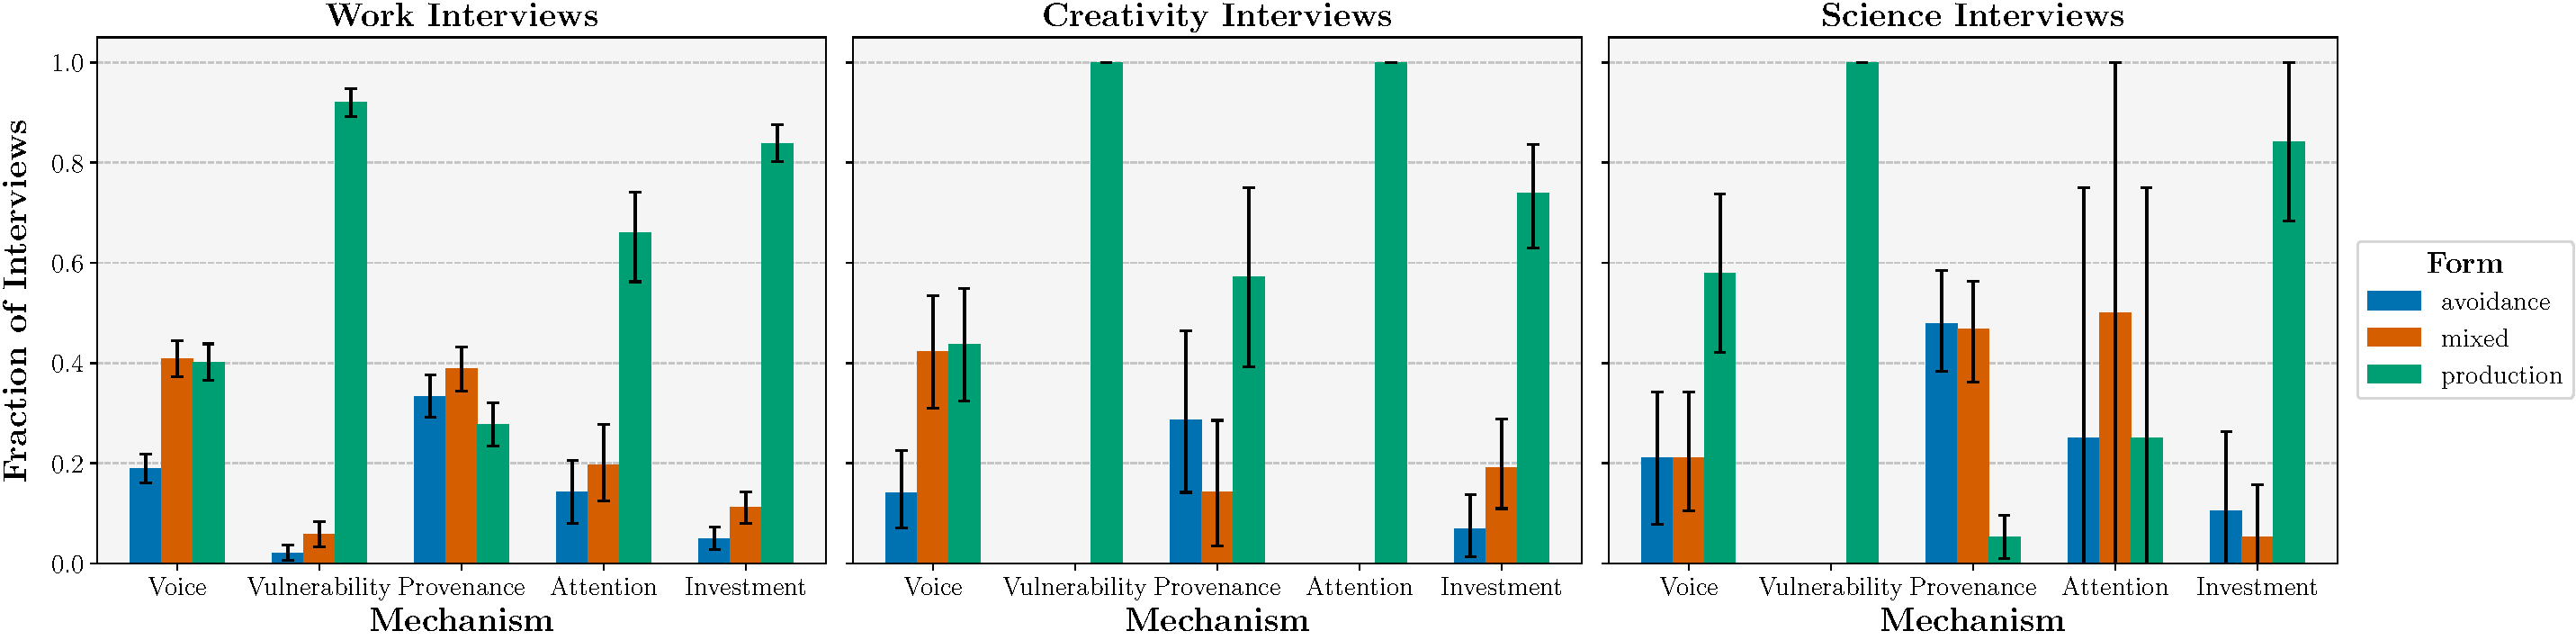
\includegraphics[width=0.9\textwidth]{figures/opacity_form.pdf}
\caption{Behavioral orientations by mechanism. Bars show fraction of cases reflecting avoidance, mixed, or production orientations.}
\label{fig:form}
\end{figure}

\subsection{Activities and Opacity Mechanisms}

To identify the work contexts in which opacity arose, we first used GPT-5.4 (with ``medium'' reasoning effort) to summarize, as a short clause, the precise task corresponding to each identified opacity mechanism and interview transcript. We embedded these descriptions with an MPNet-based sentence-transformer (\texttt{all-mpnet-base-v2}). Then, we used $k$-means to cluster embeddings separately for each opacity mechanism ($k=8$ to $18$ depending on the mechanism). Finally, we generated the cluster labels in Figure~\ref{fig:activities} by prompting GPT-5.4 to characterize each cluster given the individual activity clauses. Figure~\ref{fig:activities} displays the most common clusters by mechanism and behavioral orientation.

\begin{figure}[htbp]
\centering
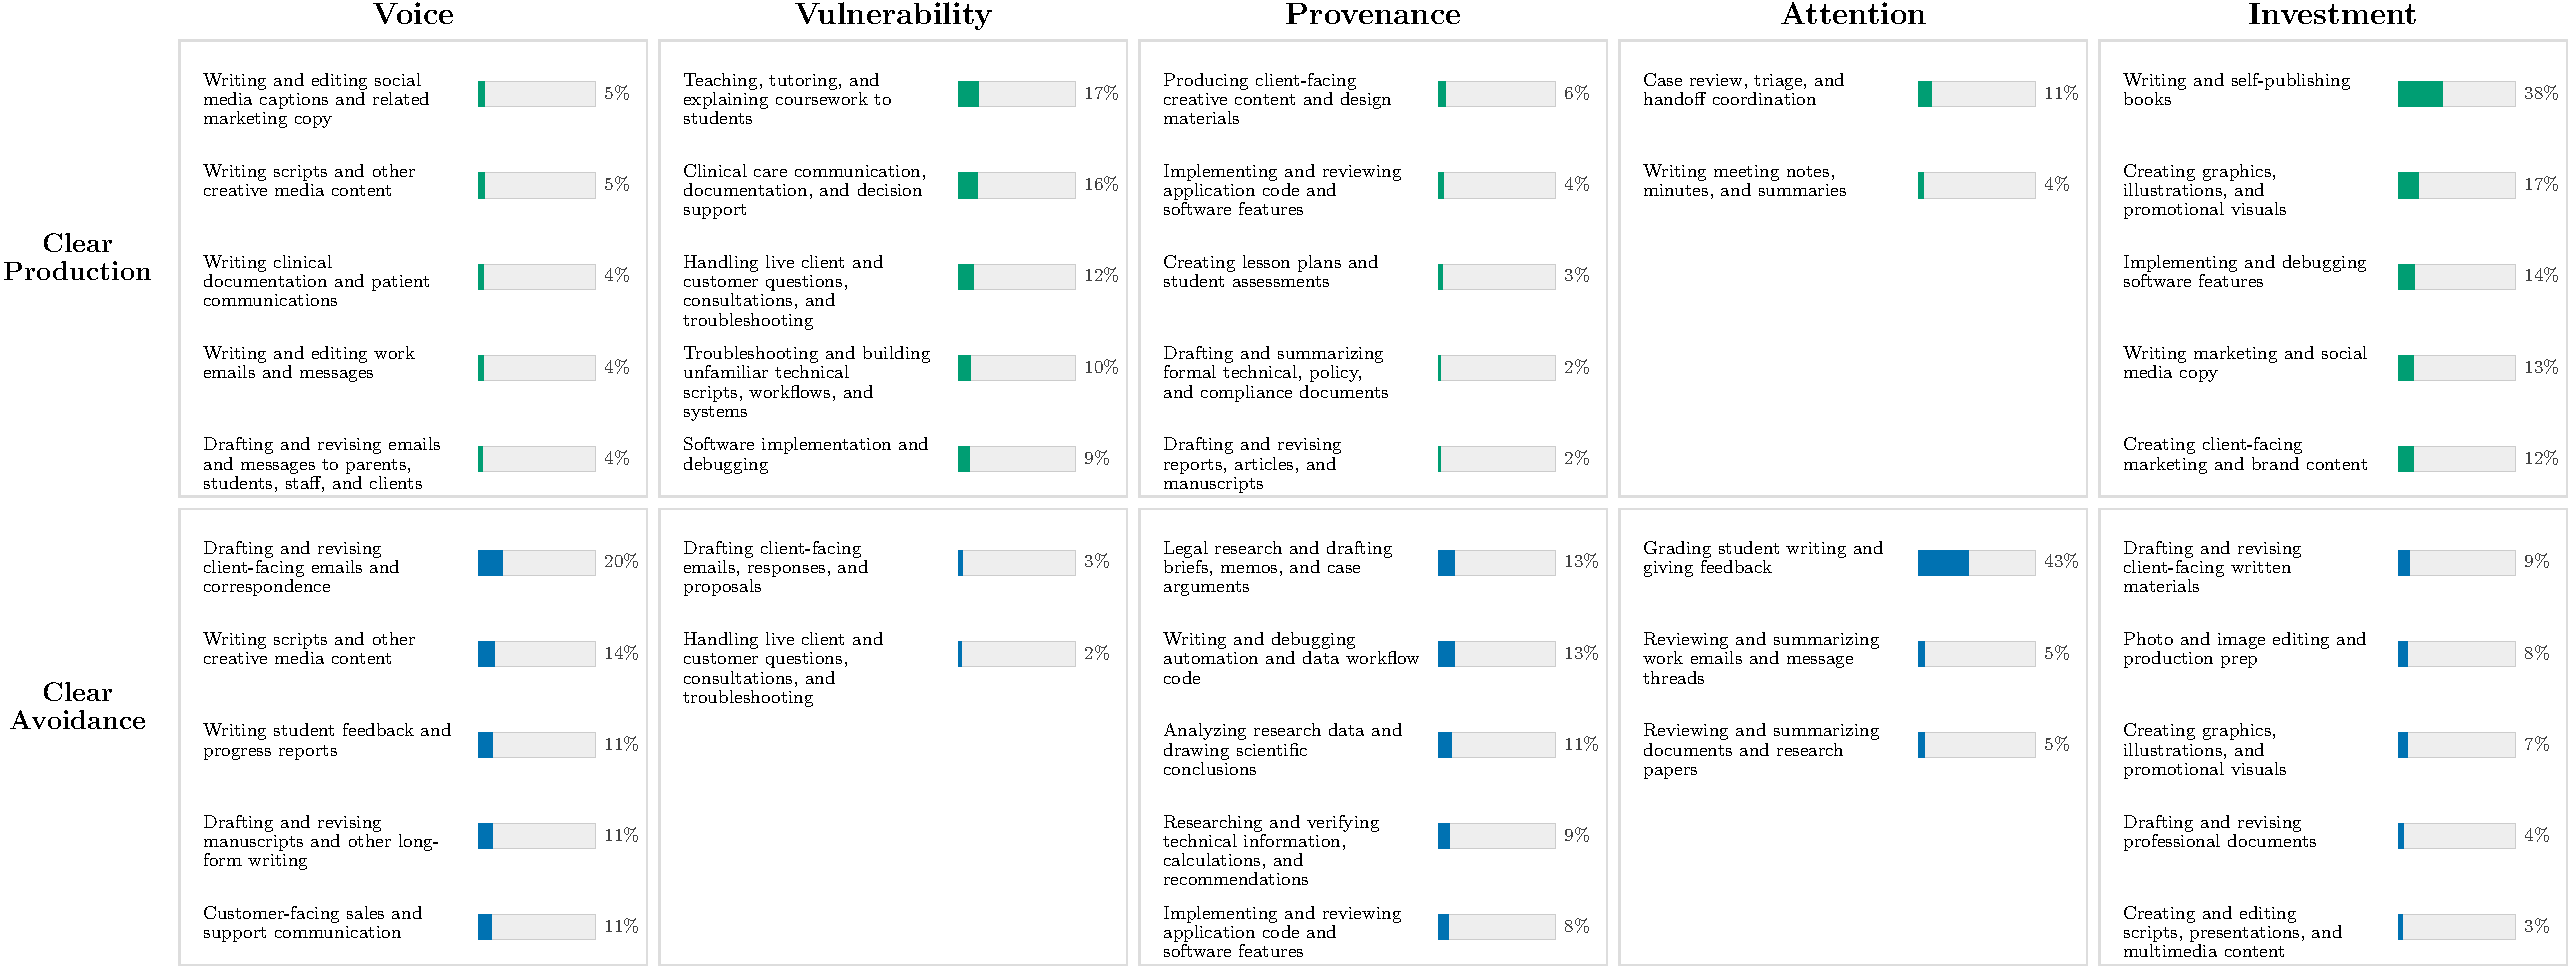
\includegraphics[width=\textwidth]{figures/tasks_opacity_mechanism_grid.pdf}
\caption{Top activity clusters by opacity mechanism and behavioral form. Bars show count of transcripts in each activity cluster.}
\label{fig:activities}
\end{figure}

Avoidance dominates only in the provenance mechanism. The close readings that follow turn to production, where the analytical innovations of our typology become most visible. 

The production of \textit{attention} opacity concentrates in case reviews, meeting documentation, and summarizing research. These are contexts where engagement can be delegated without immediate consequences. Avoidance, by contrast, is dominated by a single activity, grading student writing (43\%), where teachers refuse to let the appearance of having read substitute for actually reading. The production side reveals how the synthetic record itself becomes a site of distortion. A project lead at a software company describes how AI note-takers reshape meeting participation:

\begin{quote}
``Sometimes, people are less involved because they know they can rely on the AI to give them the meeting notes at the end. The most extreme example is not joining the call at all\ldots\ I do review the overview at the end to ensure those notes are accurate, especially if people rely on them. [The AI is] leaving tasks unassigned when they were assigned, and creating tasks for things that were just notes in the call. Lastly, the AI could miss delegating things to people as well.'' [work\_0681]
\end{quote}

AI note-takers reshape attendance through a feedback loop. Promised that the AI will capture the meeting, workers stop attending---most extremely, by ``not joining the call at all.'' But the AI's record fails in exactly the ways present participants would catch: tasks assigned go unrecorded, things mentioned get logged as commitments, delegations slip away. The fewer who attend, the fewer who can challenge the AI's account. 

The production of \textit{investment} opacity dominates across creative and professional contexts, such as self-publishing books, creating graphics and illustrations, and writing marketing copy. But the practice also occasionally scrambles the producer/avoider distinction at the heart of our typology. One speaker, transitioning from manual labor into administrative responsibilities, describes editing AI-generated reports before sending them to colleagues:

\begin{quote}
``I'll take what the AI wrote, remove any filler, change any words I wouldn't naturally use in my own speech, and heck, maybe even add in a grammatical error just so that my colleagues know I'm human and we all make mistakes. It's dangerous territory to try and appear perfect all the time because people start expecting certain standards from you, or start to look at themselves and think they're not good enough.'' [work\_0941]
\end{quote}

The inserted grammatical error mentioned by this interviewee is part of a recursive process, a sign-of-being-a-sign-of-effort. Opacity, here, is masked by a kind of counterfeit re-coupling, where producers manufacture the markers of human effort that AI-generated text otherwise lacks. Yet making AI output pass as average human text turns out to require substantial new effort, including linguistic detection of AI tells and calibrated error-insertion. Investment opacity does not eliminate labor so much as migrate it from the visible product to invisible upkeep. Notably, the participant engages in this process precisely because otherwise ``people start expecting certain standards from you.'' They produce opacity to manage the audience's future interpretive standards, on behalf of a workplace whose norms have not yet formed.

\textit{Provenance} avoidance dominates the mechanism overall and concentrates in high-accountability domains such as legal research, brief drafting, debugging automation code, and analyzing research data, where the producer's name carries subsequent consequence and defection is rare. The rare cases of provenance \textit{production}, however, reveal a structural consequence that the avoidance accounts do not. The most telling case in the corpus comes from an interviewee who is detecting it, rather than producing it. The owner of a small handyman business describes what happened when they realized their graphic designer was laundering AI output through her professional identity:

\begin{quote}
``Since I realized that our graphic designer was just using AI, I've realized that she is not choosing to think on her own about projects very much at all. I have to imagine that I'm actually prompting the AI myself, so I have to be very clear and specific with what I ask from her, as I imagine she is just copying/pasting it into some sort of AI. Really ought to just skip the middleman, to tell the truth.'' [work\_0763]
\end{quote}

The case inverts the usual perspective, as most provenance discourse is about the worker managing their own AI use, while this account is from an audience that has seen through such management. The detection does not trigger confrontation. The owner does not fire the designer, complain to her, or demand disclosure; they silently re-classify her in their own working model, moving her from a worker with judgment to \textit{middleman}, a passthrough between their instructions and the model's output. The reorganization is unilateral and undisclosed, captured in their own framing of having to ``imagine that I'm actually prompting the AI myself.'' Their framing names the footing shift directly: they now treat the AI as the author and the designer as a mere animator, with going to the AI themselves a way of cutting out the link they no longer value. Front and back stage do not collapse in any visible way. What collapses is the designer's epistemic standing in the owner's mental model of the workflow, with no occasion for repair. The closing sentence shows how provenance opacity, once detected, becomes a precursor to labor disintermediation: the worker, treated as a passthrough to AI, is silently routed around inside the workflow before any formal decision to cut her.
This rerouting will likely only be visible to the designer once her position has already eroded. Aggregated across many such silent decisions, we can see how the workplace begins to sort workers from labor inputs.

\textit{Vulnerability} opacity production appears across contexts where real-time competence displays matter, including teaching and tutoring (17\%), clinical care communication (16\%), and technical troubleshooting (10\%). It also concentrates in the early career, where the audience whose uncertainty-detection capacity is being managed is, precisely, the senior expected to detect and correct it. A medical student describes their use of OpenEvidence in exactly these terms:

\begin{quote}
``I use OpenEvidence and ask it questions as if I'm talking to a senior resident or attending and asking them questions I'm too nervous to ask in real life\ldots sometimes I use it to check over my differential or assessment and plan before presenting to my attending and it makes me feel more confident that what I'm saying makes medical sense.'' [work\_0264]
\end{quote}

The participant is replacing a person whose institutional role is to receive novice uncertainty and convert it into instruction, rather than replacing reference materials. The AI substitute is engineered to bypass the relational stakes, including embarrassment, the appearance of unpreparedness, and the small ritual humiliations through which clinical apprenticeship has historically proceeded. By using AI to ``check over'' their assessment-and-plan before presenting to the attending, they replace what was formerly a back stage encounter with a senior with a real-time pocket resource. The senior, no longer a teammate who would absorb novice questions, becomes another front stage audience they must simply perform competence to.

Vulnerability opacity is therefore a form of \textit{face-work} under conditions of automated rehearsal, in which the novice preserves the competent front before seniors by moving the risky moment of not-knowing into a private interaction with the model. Vulnerability is managed through a substitute that simulates the senior's epistemic role while stripping out the senior's recognition function. Vulnerability opacity, thus, dissolves the social occasion through which the gap would be named and addressed.

Finally, \textit{voice} avoidance concentrates in client-facing correspondence (20\%) and creative writing (14\%)---contexts where distinctive style indexes the person behind the interaction. The most theoretically revealing cases, however, are the productions routed through avoidance. An Early Years Educator, describing how they now write daily learning observations for parents, explains:

\begin{quote}
``I have fed an AI examples of my own personal observations as an example template, and the AI now uses this template to write my observations for me\ldots\ I like it to use my style of writing so that my work doesn't \textit{look} AI generated, there's a bit of stigma around it, I don't tell my colleagues that I use it\ldots\ I do worry that\ldots\ if I write my own, someone will notice the difference in quality! Which is a little silly, I did use my own language and observations as the template after all.'' [work\_0245]
\end{quote}

The participant has constructed what we might call a \textit{reflexive voice loop}. They curate a corpus of their own past front-stage performances, hand it to the model as a stylistic template, and then animate the model's outputs as their own. They remain the principal and the animator, but authorship has been displaced onto a statistical compression of their earlier self. We might call this \textit{autoventriloquism}, a form of voice opacity produced through self-impersonation with the model functioning as a stylistic mirror trained on prior performances of the self. Personhood cues like ``my style of writing'' become signs of a person who once was, reanimated in the present. Voice becomes an archived front, rather than a present expressive capacity. The audience can no longer read voice as evidence of present engagement, while the worker, having set the archived double as the standard, finds their unmediated writing falling short of it in real time.

\subsection{From Asymmetry to Inspectability}

The identity/labor asymmetry tells us which mechanisms professionals defend, but not why. Three structural features of our corpus supply the explanation. AI workplace opacity is more accurately understood as a new social organization of \textit{inspectability}, in which workers defend the signs that can be detected while routing disclosure differently across the audiences who hold them to account.
 
The first feature is a forensic asymmetry. Identity mechanisms leave detectable residue such as em-dashes and the verdicts of AI-detection software, while labor mechanisms have no comparable cue surface. There is no detector for effort that was not expended, no software that scans a finished memo for the hesitations it does not contain. A technical writer who serves multiple regulated clients articulates the resulting economy:

\begin{quote}
``They all want me to use AI, but ensure the writing cannot be detected by AI-detecting software. It is a paradoxical situation\ldots\ I tell the AI to take each citation and tell me the 1st sentence of the first body paragraph. So far, that always works.'' [work\_0240]
\end{quote}

The ``paradoxical situation'' resolves once one disaggregates audiences. Clients want prose that will not register as machine-written to the third-party detector they fear, rather than human-written prose as such. The writer therefore performs two laundering operations. Outwardly, they scrub the cue surface so the artifact passes the client's detector. Inwardly, they run their own forensic test on the AI to catch hallucinations before the client does. No comparable apparatus is contemplated for the labor the AI is doing on the article body. Hours of research and synthesis pass undetected. 
 
The same logic recurs across the corpus. An Early Years Educator deletes ``the MANY MANY em-dashes'' from their AI-generated observations because they are ``super obvious'' giveaways [work\_0245]. A developer who generated polished business descriptions reports that ``nobody seems to question the source'' [work\_0278]. A worker who ``had AI do all the work'' on a database design notes that colleagues now come to them ``for domain knowledge'' while they ``did that quite leisurely'' [work\_0693]. Where detection is possible, opacity is policed. Where it is not, opacity is produced.
 
The second feature is that this forensic substrate is itself unevenly distributed across audiences. Our cases show why workers conceal selectively---hiding AI use from managers and evaluators while remaining open with peers \citep{xia2026clever}: peers often share the same detection capacities the worker possesses, while audiences above lack them. The audience-relative pattern thus has a forensic substrate, not only a relational one. A software developer makes the segmentation explicit:

\begin{quote}
``The devs openly share features and tooling with each other. We completely hide it from management and our product people\ldots\ I didn't tell my employer that the 16 minute spike took 16 minutes. I kept the day to myself to give myself an extra long weekend.'' [work\_0747]
\end{quote}

The peer collective functions as a \textit{performance team} in Goffman's sense \citep{goffman1959presentation}, a region where fellow practitioners actively coordinate the very practice they jointly conceal from above. Mutual disclosure in the back stage enables coordinated nondisclosure on the front stage. The producer/avoider distinction collapses here. Coded in the aggregate as a producer, work\_0747 is laterally an avoider: they openly share with peers the AI use they hide from management. Orientation, in other words, is a property of the worker-audience dyad rather than of the worker alone. The same juniors who hide vulnerability from their attendings admit it ``alone with some residents or students'' [work\_0472], and the same consultants who conceal time savings from fixed-price clients share their workflow with peers [work\_0096]. What looks in the aggregate like selective stigma management is, at the relational level, coordinated audience segregation in which different audiences are entitled to different disclosures.
 
The third feature concerns how mechanisms relate to one another inside this topology. Voice delegation is the typical anchor decision, the move a participant recognizes and accounts for. An engineer articulates the cascade: ``my own skillset deteriorates if I use AI too much in that area\ldots\ I will find them much more difficult or impossible due to those skills being unused'' [work\_0012]. Once the cue surface is delegated, subsequent effects (skill atrophy, hollowed effort) accumulate as residue of a previously made decision.

\subsection{The Logic of Accounts}

LLM-assisted coding captures prevalence and behavioral orientation, but accounts also reveal \textit{practical reasoning}, the way professionals justify their practices \citep{scott1968accounts}. As described above, we hand-coded 207 cases for accountability- and efficiency-oriented justifications, which are not mutually exclusive.
 
Accountability justifications appeared in 56.5\% of cases, efficiency in 34.3\%. Justification type varied sharply by behavioral orientation and by mechanism (Figure~\ref{fig:justifications}). 93.7\% of avoidance cases contained accountability justifications, compared to only 20.6\% of production cases. Accountability justifications appeared in 78.3\% of voice cases and 71.4\% of provenance cases, but in only 22.0\% of vulnerability cases and 30.3\% of investment cases.

\begin{figure}[htbp]
\centering
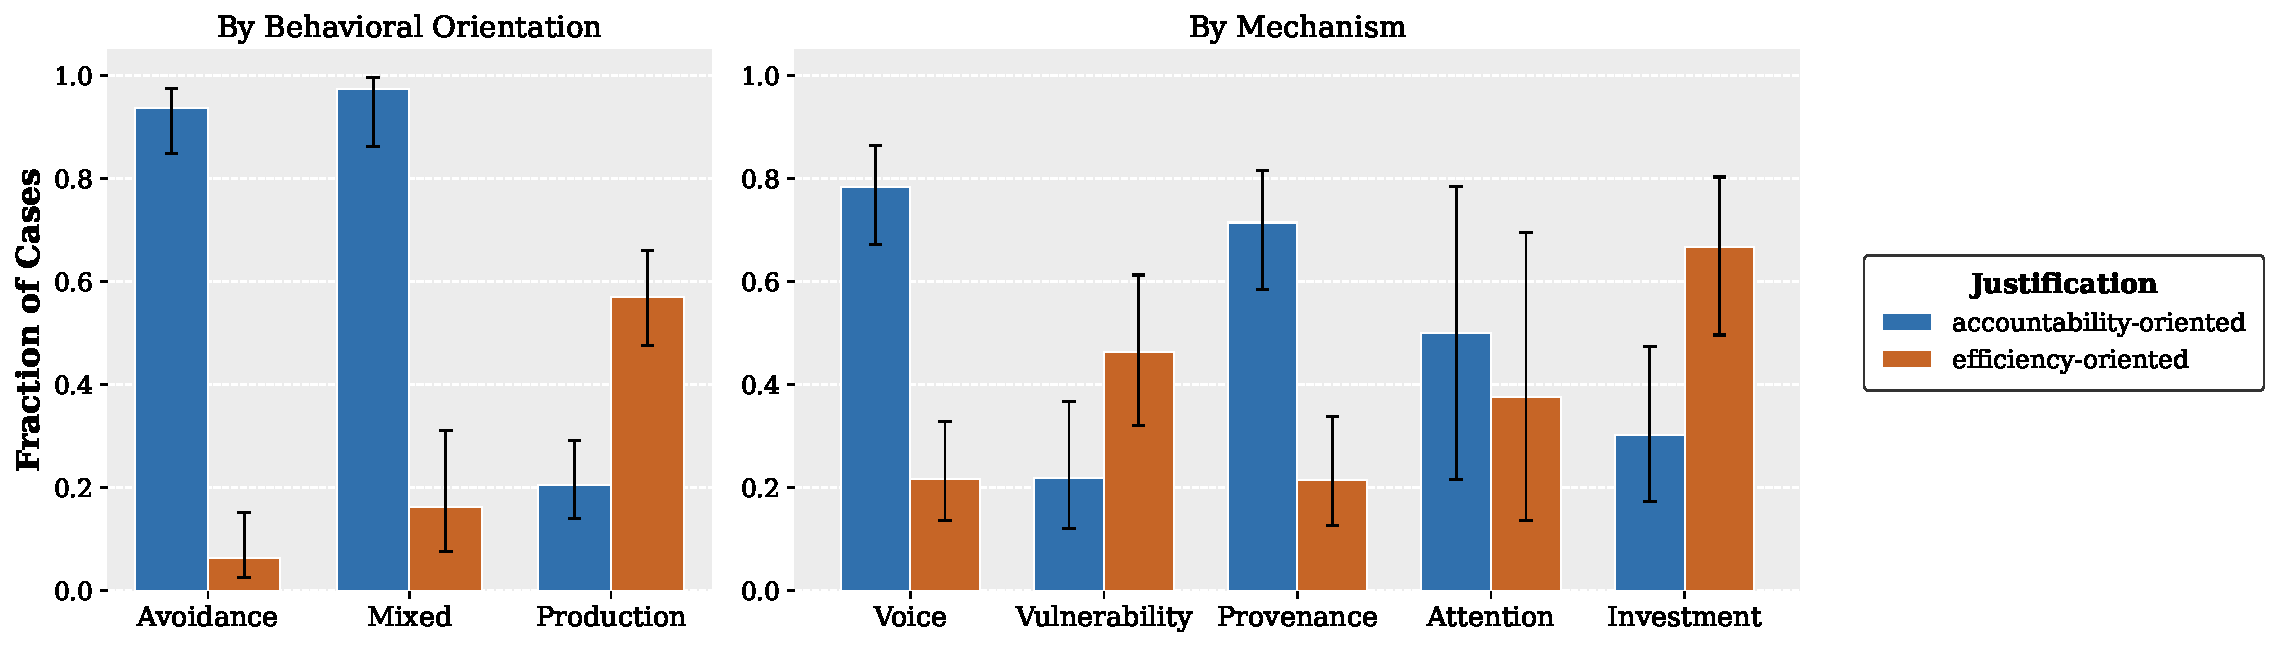
\includegraphics[width=\textwidth]{figures/justifications.pdf}
\caption{Justification types across hand-coded cases ($n = 207$). Bars show the fraction of cases containing accountability-oriented and efficiency-oriented justifications. Categories are not mutually exclusive. Error bars are 95\% Wilson confidence intervals.}
\label{fig:justifications}
\end{figure}

A freelance editor illustrates how both justification types can operate in a single account:

\begin{quote}
``If I feel like that is how the text should read, I will use AI's suggestion. I prefer to blend the work as I feel like I'm cheating a bit otherwise. The author is paying me to edit their work, so using AI sometimes feels like the easy route. I know that the author wouldn't be able to edit their own work, even using AI, as it is a skill.'' [work\_0361]
\end{quote}

The editor invokes professional obligation (``the author is paying me''), acknowledges efficiency gains (``the easy route''), and resolves the tension by reasserting that editing ``is a skill.'' Accountability and efficiency justifications coexist when the worker can claim the labor as their own expertise.
 
The general finding behind this asymmetry is more consequential than any single case. Resisting AI use in efficiency-oriented workplaces is untoward and must be accounted for through responsibility, liability, or trust, while producing labor opacity passes without comment. Efficiency has become the unmarked moral default; what requires explanation is the refusal to obscure effort, not the obscuring itself.
 
This reflexivity asymmetry recurs at the salience level. Workers articulate opacity most explicitly for voice (40\% of voice-present cases are coded as ``clear'' rather than ``potential'') and least for vulnerability (12\%) and attention (16\%). When AI fills in for uncertainty or attendance, workers describe it as workflow efficiency---``I turn to AI when I'm stuck,'' ``I let AI handle the meeting notes''---without naming the social work being done. Reflexivity, in other words, tracks vocabulary: workers recognize and defend opacity practices their workplace already names. They produce, often without noticing, the practices it does not. 

% ============================================================================
% DISCUSSION
% ============================================================================
\section{Discussion}

AI use is reorganizing three structural conditions of workplace performance, each paired with a normative asymmetry in how workers respond. We discuss these in turn before turning to what they imply for governance.
 
First, AI use removes the social occasions through which professional standing gets repaired and developed. When AI use is detected, the audience reclassifies the worker silently rather than challenging them and demanding repair. Concealment removes not just the cue surface but the relational moment through which suspicion becomes repair, uncertainty becomes instruction, or attendance becomes commitment. What workers lose first is not face, but position.
 
Second, voice has begun to function as an archive marker rather than as a present-self expression. Goffman's animator/author/principal triad \citep{goffman1981forms} usually splits across different people. Here it splits across different versions of the same person across time. The present-day animator and principal speak for an author who is an archived version of the worker's earlier self. The work of producing voice shifts backward in time, from the moment of writing to the earlier moment of choosing which past writing to feed the model. Voice work becomes archive maintenance.
 
Third, the many small impression-management decisions of workplace life have compressed into one originating choice. Voice delegation is the primary move that workers recognize and account for, while vulnerability, attention, and investment opacity follow automatically.
 
These structural shifts come paired with a normative asymmetry. The avoidance of opacity requires justification through responsibility, liability, or professional duty, while it is often produced without comment as ambient workflow efficiency. GenAI is obscuring uncertainty, simulating attendance, and detaching effort from output that workplace discourse has not yet named, and workers cannot strategize about what they cannot articulate.

\subsection{Limitations}

Several limitations bound the present account. First, the corpus is itself a recruited and AI-mediated artifact. Participants were drawn from crowdworker platforms and interviewed by Claude rather than by a human researcher, which likely shapes both who consented and what they disclosed. Disclosing AI use to an AI interviewer is not interactionally equivalent to disclosing it to a manager, and the framing of the interviewer as an AI may have lowered the social cost of acknowledging AI use. Self-report data, here as elsewhere, gives access to professionals' accounts of practice rather than to practice itself, and our analysis should be read accordingly. Second, the three subsamples are unbalanced: the general workforce ($n = 1{,}000$) dominates the corpus and the creative and scientific samples ($n = 125$ each) are heterogeneous within themselves. The domain-level comparisons in \S 4.1 are best understood as broad-strokes contrasts rather than fine-grained occupational claims. Third, our primary coding was conducted by a large language model (GPT-5.4) against a rubric we developed iteratively. While we hand-coded a stratified subsample of 207 cases for justification type, we did not run a second human coder over the LLM's salience and behavioral-orientation assignments, and the IRR statistics typically reported for hand-coded qualitative data are therefore unavailable. The coding sheet, prompts, and full set of LLM-generated labels are released alongside this paper so that subsequent work can validate, contest, or extend them.

Effort opacity, we have argued, is an audience-sensitive sorting mechanism in which workers protect identity cues and release labor cues. The professionals who gain most from AI in their early careers also face the strongest pressure to conceal it. They resolve this double bind by routing disclosure differently across audiences and by treating each downstream consequence as ambient rather than as a decision worth accounting for. If the pattern persists, the human role at work will be redefined as an accountable front for outputs generated through increasingly opaque sociotechnical processes, with institutional expectations and actual practice growing steadily out of alignment. Governance frameworks built on universal disclosure will be insufficient to catch these developments. What is needed is a clear sense of which forms of human involvement must remain inspectable, and to whom.

\section*{Data and Code Availability}

The Anthropic Interviewer transcripts analyzed in this paper are publicly available under CC-BY at \url{https://huggingface.co/datasets/Anthropic/AnthropicInterviewer}. All analysis code, LLM coding prompts, the hand-coded justification sheet, and the figure-generation scripts used to produce the results reported here are released at \url{https://github.com/dlab-projects/fabricated_front}.

\bibliography{sn-bibliography}% common bib file
%% if required, the content of .bbl file can be included here once bbl is generated
%%\input sn-article.bbl

\end{document}
